\section{Computation Review}
\begin{frame}{Computation Review}
\begin{itemize}
\item use factorisation theorem: PDF and $s=\xi S_h$
\item PGF: $\Pg(k_1) + \Pggx(q) \to \PaQ(p_2) + \PQ(p_1)$
\item three massive particles: $m^2>0,q^2=-Q^2<0$
\item<2-> compute 2-to-3-phase space: e.g. $dPS_3 \sim dt_1du_1d\Omega_nd\hat{\mathcal{I}}$ \iRef{Laenen, Bojak}
\item<2-> diagrams: %
\raisebox{-.4\height}{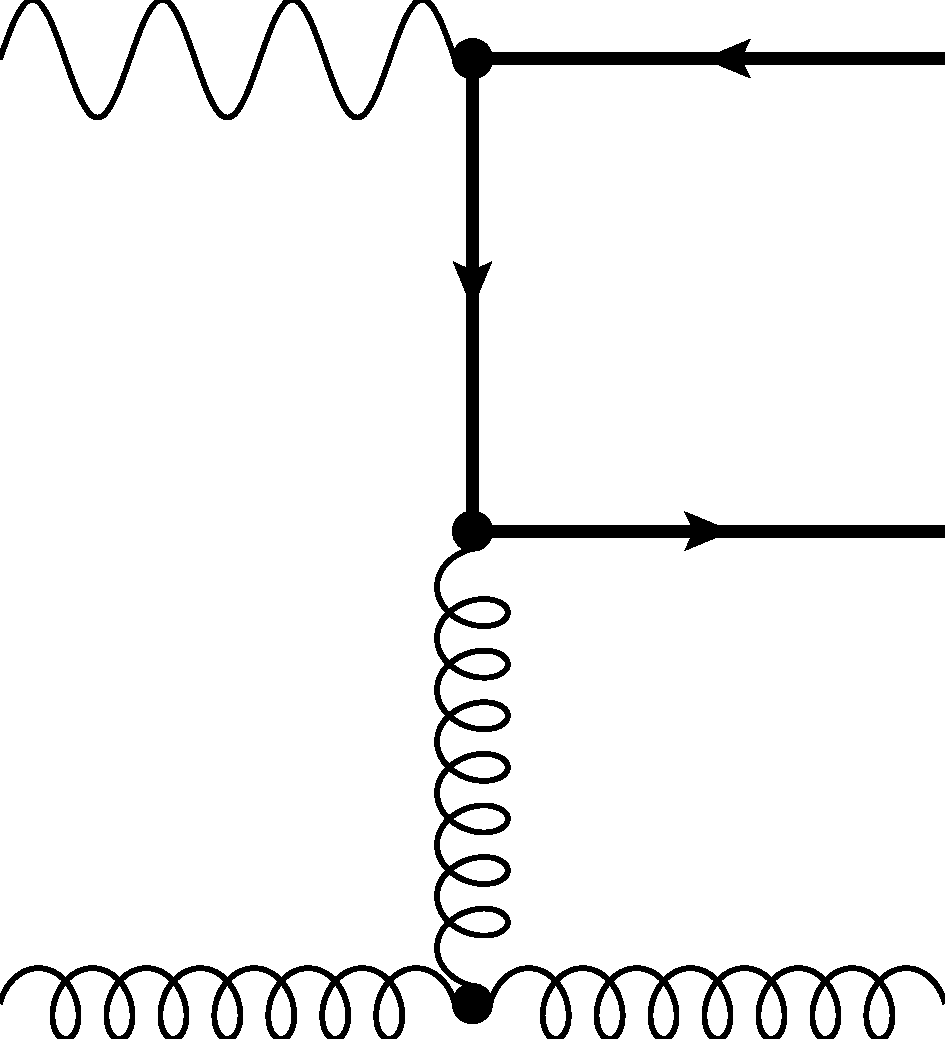
\includegraphics[height=.19\textheight]{img/nlo-g-4}} +%
\raisebox{-.4\height}{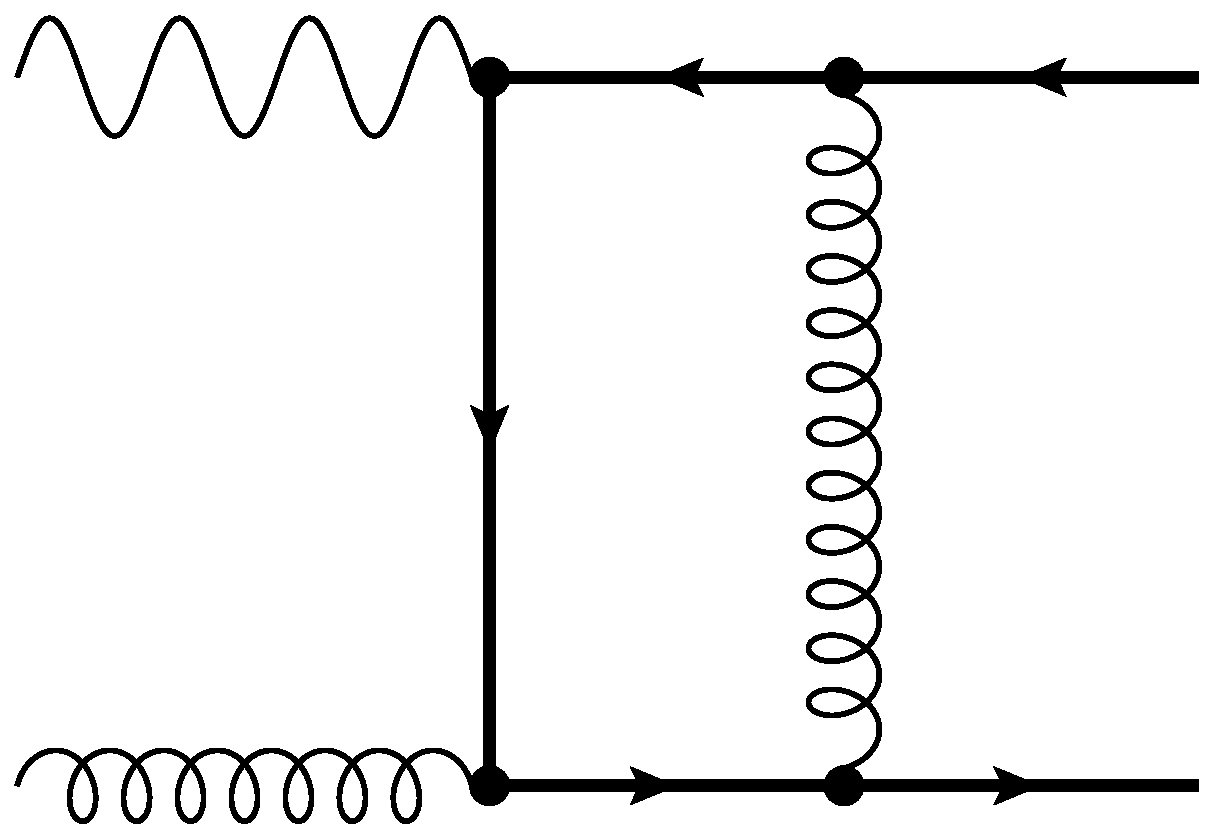
\includegraphics[height=.19\textheight]{img/nlo-v-1}} + %
\raisebox{-.4\height}{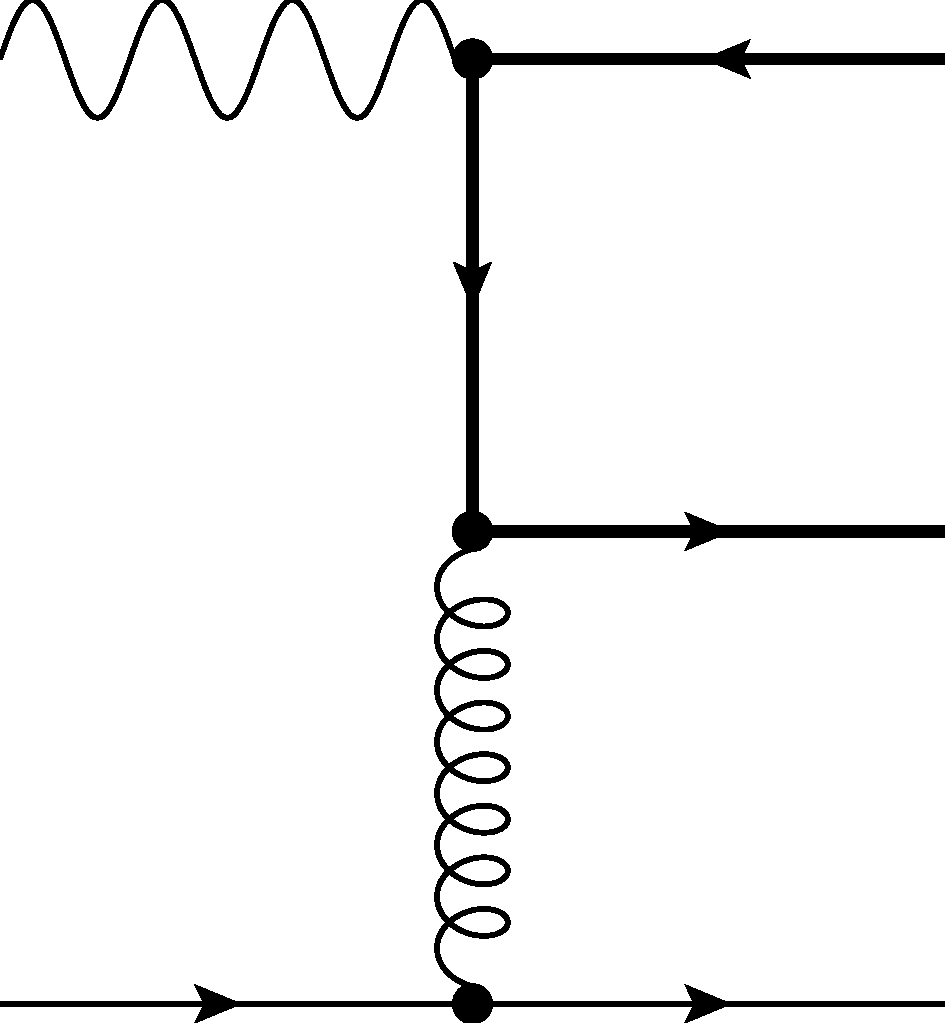
\includegraphics[height=.19\textheight]{img/nlo-q-1}} + %
\raisebox{-.4\height}{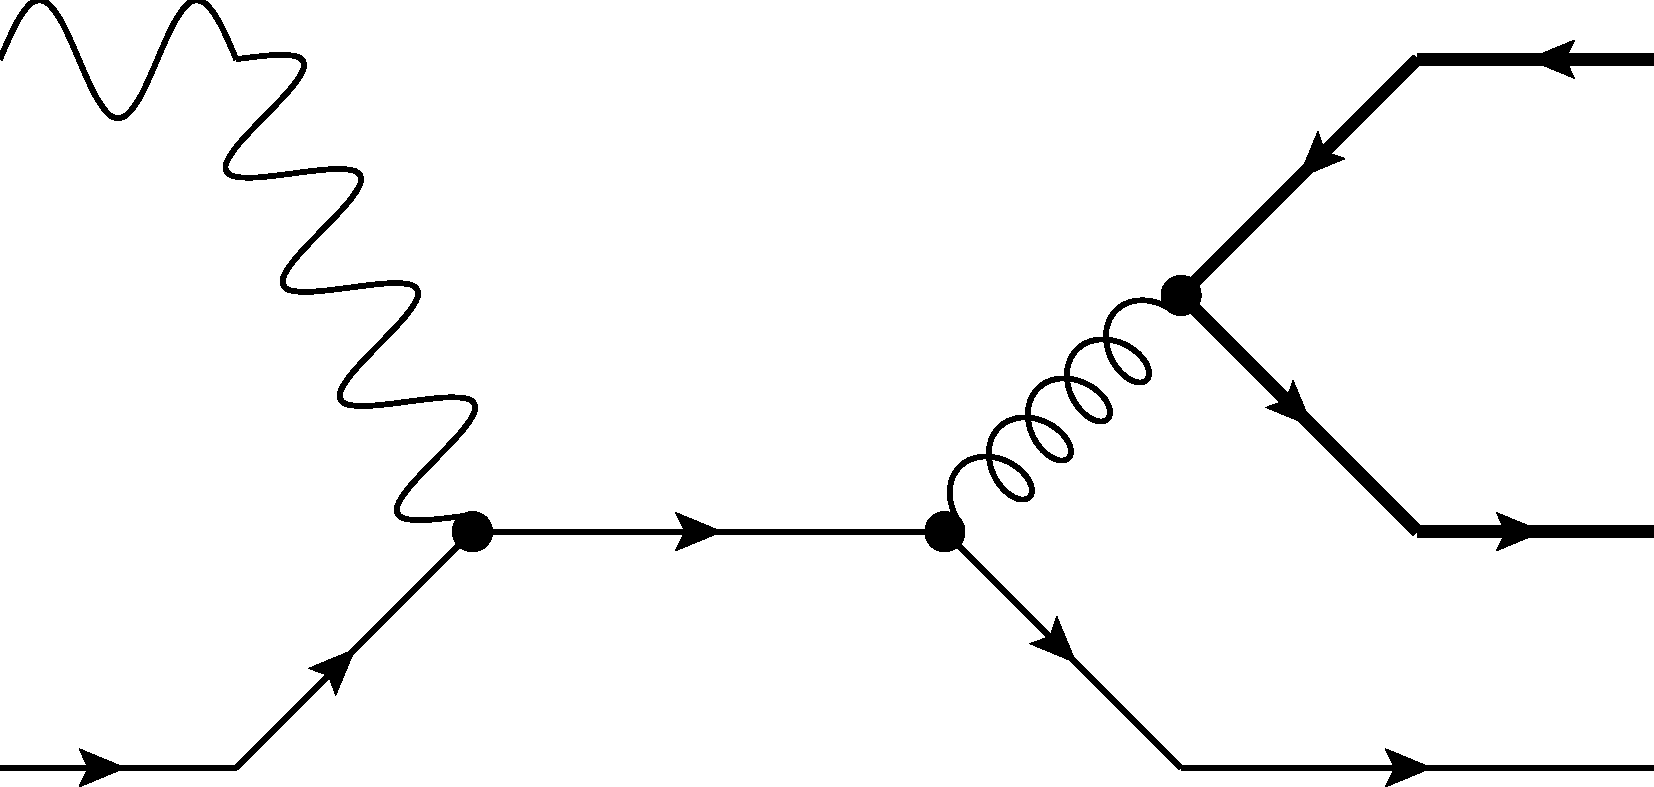
\includegraphics[height=.19\textheight]{pyfeyn2/nlo-q-4}} + \ldots
\item<3-> collinear poles $\to$ mass factorization ($\MSbar$)
\item<3-> soft + virtual + renormalization ($\MSbar_m$) + factorization is finite \iRef{Laenen,Bojak}
\item<4-> $\gamma_5$ and $\varepsilon_{\mu\nu\rho\sigma}$ in $n$-dimension? $\to$ HVBM scheme \iRef{'t Hooft,Veltman,Breitenlohner,Maison}
\end{itemize}
\end{frame}
